\documentclass[twoside]{book}

% Packages required by doxygen
\usepackage{fixltx2e}
\usepackage{calc}
\usepackage{doxygen}
\usepackage[export]{adjustbox} % also loads graphicx
\usepackage{graphicx}
\usepackage[utf8]{inputenc}
\usepackage{makeidx}
\usepackage{multicol}
\usepackage{multirow}
\PassOptionsToPackage{warn}{textcomp}
\usepackage{textcomp}
\usepackage[nointegrals]{wasysym}
\usepackage[table]{xcolor}

% Font selection
\usepackage[T1]{fontenc}
\usepackage[scaled=.90]{helvet}
\usepackage{courier}
\usepackage{amssymb}
\usepackage{sectsty}
\renewcommand{\familydefault}{\sfdefault}
\allsectionsfont{%
  \fontseries{bc}\selectfont%
  \color{darkgray}%
}
\renewcommand{\DoxyLabelFont}{%
  \fontseries{bc}\selectfont%
  \color{darkgray}%
}
\newcommand{\+}{\discretionary{\mbox{\scriptsize$\hookleftarrow$}}{}{}}

% Page & text layout
\usepackage{geometry}
\geometry{%
  a4paper,%
  top=2.5cm,%
  bottom=2.5cm,%
  left=2.5cm,%
  right=2.5cm%
}
\tolerance=750
\hfuzz=15pt
\hbadness=750
\setlength{\emergencystretch}{15pt}
\setlength{\parindent}{0cm}
\setlength{\parskip}{0.2cm}
\makeatletter
\renewcommand{\paragraph}{%
  \@startsection{paragraph}{4}{0ex}{-1.0ex}{1.0ex}{%
    \normalfont\normalsize\bfseries\SS@parafont%
  }%
}
\renewcommand{\subparagraph}{%
  \@startsection{subparagraph}{5}{0ex}{-1.0ex}{1.0ex}{%
    \normalfont\normalsize\bfseries\SS@subparafont%
  }%
}
\makeatother

% Headers & footers
\usepackage{fancyhdr}
\pagestyle{fancyplain}
\fancyhead[LE]{\fancyplain{}{\bfseries\thepage}}
\fancyhead[CE]{\fancyplain{}{}}
\fancyhead[RE]{\fancyplain{}{\bfseries\leftmark}}
\fancyhead[LO]{\fancyplain{}{\bfseries\rightmark}}
\fancyhead[CO]{\fancyplain{}{}}
\fancyhead[RO]{\fancyplain{}{\bfseries\thepage}}
\fancyfoot[LE]{\fancyplain{}{}}
\fancyfoot[CE]{\fancyplain{}{}}
\fancyfoot[RE]{\fancyplain{}{\bfseries\scriptsize Generated on Tue Oct 6 2015 20\+:27\+:19 for B\+A\+R\+E\+S by Doxygen }}
\fancyfoot[LO]{\fancyplain{}{\bfseries\scriptsize Generated on Tue Oct 6 2015 20\+:27\+:19 for B\+A\+R\+E\+S by Doxygen }}
\fancyfoot[CO]{\fancyplain{}{}}
\fancyfoot[RO]{\fancyplain{}{}}
\renewcommand{\footrulewidth}{0.4pt}
\renewcommand{\chaptermark}[1]{%
  \markboth{#1}{}%
}
\renewcommand{\sectionmark}[1]{%
  \markright{\thesection\ #1}%
}

% Indices & bibliography
\usepackage{natbib}
\usepackage[titles]{tocloft}
\setcounter{tocdepth}{3}
\setcounter{secnumdepth}{5}
\makeindex

% Hyperlinks (required, but should be loaded last)
\usepackage{ifpdf}
\ifpdf
  \usepackage[pdftex,pagebackref=true]{hyperref}
\else
  \usepackage[ps2pdf,pagebackref=true]{hyperref}
\fi
\hypersetup{%
  colorlinks=true,%
  linkcolor=blue,%
  citecolor=blue,%
  unicode%
}

% Custom commands
\newcommand{\clearemptydoublepage}{%
  \newpage{\pagestyle{empty}\cleardoublepage}%
}

\usepackage{caption}
\captionsetup{labelsep=space,justification=centering,font={bf},singlelinecheck=off,skip=4pt,position=top}

%===== C O N T E N T S =====

\begin{document}

% Titlepage & ToC
\hypersetup{pageanchor=false,
             bookmarks=true,
             bookmarksnumbered=true,
             pdfencoding=unicode
            }
\pagenumbering{roman}
\begin{titlepage}
\vspace*{7cm}
\begin{center}%
{\Large B\+A\+R\+ES \\[1ex]\large 1 }\\
\vspace*{1cm}
{\large Generated by Doxygen 1.8.11}\\
\vspace*{0.5cm}
{\small Tue Oct 6 2015 20:27:19}\\
\end{center}
\end{titlepage}
\clearemptydoublepage
\tableofcontents
\clearemptydoublepage
\pagenumbering{arabic}
\hypersetup{pageanchor=true}

%--- Begin generated contents ---
\chapter{Namespace Index}
\section{Namespace List}
Here is a list of all documented namespaces with brief descriptions\+:\begin{DoxyCompactList}
\item\contentsline{section}{\hyperlink{namespaceGreati}{Greati} \\*Indicates classes constructed by Vitor \hyperlink{namespaceGreati}{Greati} }{\pageref{namespaceGreati}}{}
\end{DoxyCompactList}

\chapter{Hierarchical Index}
\section{Class Hierarchy}
This inheritance list is sorted roughly, but not completely, alphabetically\+:\begin{DoxyCompactList}
\item \contentsline{section}{Abs\+Stack$<$ Object $>$}{\pageref{classAbsStack}}{}
\begin{DoxyCompactList}
\item \contentsline{section}{Stack$<$ Object $>$}{\pageref{classStack}}{}
\end{DoxyCompactList}
\item \contentsline{section}{Bares}{\pageref{classBares}}{}
\item \contentsline{section}{Bares\+:\+:Error}{\pageref{structBares_1_1Error}}{}
\item \contentsline{section}{Queue$<$ Data $>$}{\pageref{classQueue}}{}
\item \contentsline{section}{Bares\+:\+:Token}{\pageref{structBares_1_1Token}}{}
\item \contentsline{section}{Greati\+:\+:Vector$<$ T $>$}{\pageref{classGreati_1_1Vector}}{}
\item \contentsline{section}{Greati\+:\+:Vector$<$ Bares\+:\+:Error $>$}{\pageref{classGreati_1_1Vector}}{}
\end{DoxyCompactList}

\chapter{Class Index}
\section{Class List}
Here are the classes, structs, unions and interfaces with brief descriptions\+:\begin{DoxyCompactList}
\item\contentsline{section}{\hyperlink{classAbsStack}{Abs\+Stack$<$ Object $>$} \\*Abstract class for \hyperlink{classStack}{Stack} implementation }{\pageref{classAbsStack}}{}
\item\contentsline{section}{\hyperlink{classBares}{Bares} \\*Main class of B\+A\+R\+ES }{\pageref{classBares}}{}
\item\contentsline{section}{\hyperlink{structBares_1_1Error}{Bares\+::\+Error} \\*This struct is instanciated when an error is detected. It has a code and the problematic token }{\pageref{structBares_1_1Error}}{}
\item\contentsline{section}{\hyperlink{classQueue}{Queue$<$ Data $>$} \\*\hyperlink{classQueue}{Queue} implementation }{\pageref{classQueue}}{}
\item\contentsline{section}{\hyperlink{classStack}{Stack$<$ Object $>$} \\*Implementation of a stack }{\pageref{classStack}}{}
\item\contentsline{section}{\hyperlink{structBares_1_1Token}{Bares\+::\+Token} \\*Struct that represents each element inside an expression. It can be an operand or an operator }{\pageref{structBares_1_1Token}}{}
\item\contentsline{section}{\hyperlink{classGreati_1_1Vector}{Greati\+::\+Vector$<$ T $>$} \\*A simple Array\+List implementation }{\pageref{classGreati_1_1Vector}}{}
\end{DoxyCompactList}

\chapter{Namespace Documentation}
\hypertarget{namespaceGreati}{}\section{Greati Namespace Reference}
\label{namespaceGreati}\index{Greati@{Greati}}


Indicates classes constructed by Vitor \hyperlink{namespaceGreati}{Greati}.  


\subsection*{Classes}
\begin{DoxyCompactItemize}
\item 
class \hyperlink{classGreati_1_1Vector}{Vector}
\begin{DoxyCompactList}\small\item\em A simple Array\+List implementation. \end{DoxyCompactList}\end{DoxyCompactItemize}


\subsection{Detailed Description}
Indicates classes constructed by Vitor \hyperlink{namespaceGreati}{Greati}. 
\chapter{Class Documentation}
\hypertarget{classAbsStack}{}\section{Abs\+Stack$<$ Object $>$ Class Template Reference}
\label{classAbsStack}\index{Abs\+Stack$<$ Object $>$@{Abs\+Stack$<$ Object $>$}}


Abstract class for \hyperlink{classStack}{Stack} implementation.  




{\ttfamily \#include $<$Abs\+Stack.\+h$>$}

Inheritance diagram for Abs\+Stack$<$ Object $>$\+:\begin{figure}[H]
\begin{center}
\leavevmode
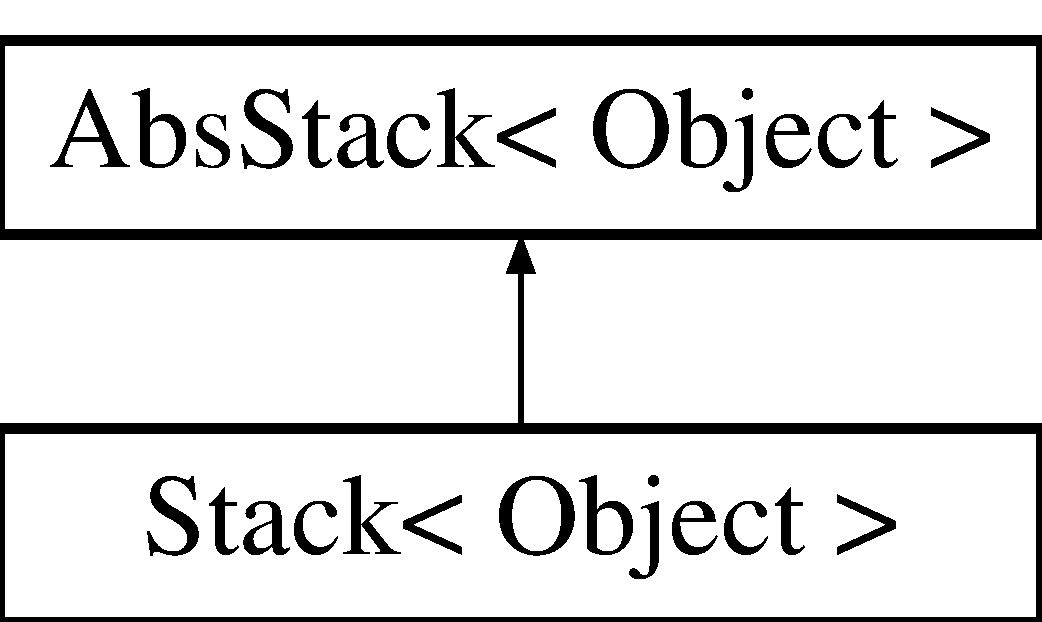
\includegraphics[height=2.000000cm]{classAbsStack}
\end{center}
\end{figure}
\subsection*{Public Member Functions}
\begin{DoxyCompactItemize}
\item 
virtual void {\bfseries push} (const Object \&x)=0\hypertarget{classAbsStack_ace9c9f220a85a96e3202af54356a8e26}{}\label{classAbsStack_ace9c9f220a85a96e3202af54356a8e26}

\item 
virtual const Object \& {\bfseries pop} ()=0\hypertarget{classAbsStack_ab80d724cba47bb4d8a399ceb123404dd}{}\label{classAbsStack_ab80d724cba47bb4d8a399ceb123404dd}

\item 
virtual const Object \& {\bfseries top} () const  =0\hypertarget{classAbsStack_aec836c9b4b5a9c58ab86ead63455e01a}{}\label{classAbsStack_aec836c9b4b5a9c58ab86ead63455e01a}

\item 
virtual bool {\bfseries empty} () const  =0\hypertarget{classAbsStack_afa498b68fa8516acf9c25d833583bf82}{}\label{classAbsStack_afa498b68fa8516acf9c25d833583bf82}

\item 
virtual void {\bfseries clear} ()=0\hypertarget{classAbsStack_a141d50ead5311933b7ab711b4d3d4cb0}{}\label{classAbsStack_a141d50ead5311933b7ab711b4d3d4cb0}

\end{DoxyCompactItemize}
\subsection*{Private Member Functions}
\begin{DoxyCompactItemize}
\item 
{\bfseries Abs\+Stack} (const \hyperlink{classAbsStack}{Abs\+Stack} \&)\hypertarget{classAbsStack_a325df7f03f0dca13168400acc29d7690}{}\label{classAbsStack_a325df7f03f0dca13168400acc29d7690}

\end{DoxyCompactItemize}


\subsection{Detailed Description}
\subsubsection*{template$<$class Object$>$\\*
class Abs\+Stack$<$ Object $>$}

Abstract class for \hyperlink{classStack}{Stack} implementation. 


\begin{DoxyPre}
SOURCE FILE : \hyperlink{AbsStack_8h_source}{AbsStack.h}
DESCRIPTION.: \hyperlink{classStack}{Stack} abstract class interface - no implementation.
AUTHOR......: Selan R. dos Santos
LOCATION....: DIMAp/UFRN.
SATARTED ON.: August/2005
CHANGES.....: None.\end{DoxyPre}



\begin{DoxyPre}TO COMPILE..: Not to be compiled.
OBS.........: Part of the LP1 Project.\end{DoxyPre}



\begin{DoxyPre}LAST UPDATE.: March 8th, 2007.
LAST UPDATE.: April tth, 2015.
\end{DoxyPre}
 \begin{DoxyAuthor}{Author}
Selan R. dos Santos. 
\end{DoxyAuthor}


The documentation for this class was generated from the following file\+:\begin{DoxyCompactItemize}
\item 
include/Abs\+Stack.\+h\end{DoxyCompactItemize}

\hypertarget{classBares}{}\section{Bares Class Reference}
\label{classBares}\index{Bares@{Bares}}


Main class of B\+A\+R\+ES.  




{\ttfamily \#include $<$bares.\+h$>$}

\subsection*{Classes}
\begin{DoxyCompactItemize}
\item 
struct \hyperlink{structBares_1_1Error}{Error}
\begin{DoxyCompactList}\small\item\em This struct is instanciated when an error is detected. It has a code and the problematic token. \end{DoxyCompactList}\item 
struct \hyperlink{structBares_1_1Token}{Token}
\begin{DoxyCompactList}\small\item\em Struct that represents each element inside an expression. It can be an operand or an operator. \end{DoxyCompactList}\end{DoxyCompactItemize}
\subsection*{Public Types}
\begin{DoxyCompactItemize}
\item 
enum \hyperlink{classBares_ad484a97e0efc1721d2b95209a1700e44}{Error\+Code} \{ \\*
\hyperlink{classBares_ad484a97e0efc1721d2b95209a1700e44a077915ac2c681ed3c2e5143fa6855abc}{Error\+Code\+::\+I\+N\+V\+A\+L\+I\+D\+\_\+\+N\+U\+M\+B\+ER} = 1, 
\hyperlink{classBares_ad484a97e0efc1721d2b95209a1700e44ae8480abe361722c6fc560d57a8751712}{Error\+Code\+::\+L\+A\+C\+K\+I\+N\+G\+\_\+\+O\+P\+E\+R\+A\+ND}, 
\hyperlink{classBares_ad484a97e0efc1721d2b95209a1700e44a6bf179afa8f7fba18cf39bc0ca6fe043}{Error\+Code\+::\+I\+N\+V\+A\+L\+I\+D\+\_\+\+O\+P\+E\+R\+A\+ND}, 
\hyperlink{classBares_ad484a97e0efc1721d2b95209a1700e44a29b8e189abb3870e81dcf17ffcbf1f31}{Error\+Code\+::\+I\+N\+V\+A\+L\+I\+D\+\_\+\+O\+P\+E\+R\+A\+T\+OR}, 
\\*
\hyperlink{classBares_ad484a97e0efc1721d2b95209a1700e44a22bca2cdebe774eae0632624429e990d}{Error\+Code\+::\+L\+A\+C\+K\+I\+N\+G\+\_\+\+O\+P\+E\+R\+A\+T\+OR}, 
\hyperlink{classBares_ad484a97e0efc1721d2b95209a1700e44a9f3ccb0df8d33fb668e9473f6bd04a35}{Error\+Code\+::\+I\+N\+V\+A\+L\+I\+D\+\_\+\+S\+C\+O\+P\+E\+\_\+\+C\+L\+O\+SE}, 
\hyperlink{classBares_ad484a97e0efc1721d2b95209a1700e44ae664084bba857b2c43cb86f844efdb04}{Error\+Code\+::\+U\+N\+C\+L\+O\+S\+E\+D\+\_\+\+S\+C\+O\+PE}, 
\hyperlink{classBares_ad484a97e0efc1721d2b95209a1700e44a5e807fe8929e4974ec886390b3832033}{Error\+Code\+::\+D\+I\+V\+I\+S\+I\+O\+N\+\_\+\+B\+Y\+\_\+\+Z\+E\+RO}
 \}\begin{DoxyCompactList}\small\item\em Enum that contains codes representing all kinds of errors that can happen. It\textquotesingle{}s used to select the correct message to be displayed when the error occur. \end{DoxyCompactList}
\item 
enum \hyperlink{classBares_a656cd507b0ddaa049dc7e6548459b6d8}{Type\+Symbol} \{ \hyperlink{classBares_a656cd507b0ddaa049dc7e6548459b6d8a11f3de9b2b548c31805cf34d512ee177}{Type\+Symbol\+::\+O\+P\+E\+R\+A\+ND}, 
\hyperlink{classBares_a656cd507b0ddaa049dc7e6548459b6d8a986496ca5b23669b8661171566a167c3}{Type\+Symbol\+::\+O\+P\+E\+R\+A\+T\+OR}, 
\hyperlink{classBares_a656cd507b0ddaa049dc7e6548459b6d8a6bf179afa8f7fba18cf39bc0ca6fe043}{Type\+Symbol\+::\+I\+N\+V\+A\+L\+I\+D\+\_\+\+O\+P\+E\+R\+A\+ND}, 
\hyperlink{classBares_a656cd507b0ddaa049dc7e6548459b6d8a29b8e189abb3870e81dcf17ffcbf1f31}{Type\+Symbol\+::\+I\+N\+V\+A\+L\+I\+D\+\_\+\+O\+P\+E\+R\+A\+T\+OR}
 \}\begin{DoxyCompactList}\small\item\em Enum that represents possible types of symbols. It\textquotesingle{}s used in verifications and to classify tokens. \end{DoxyCompactList}
\end{DoxyCompactItemize}
\subsection*{Public Member Functions}
\begin{DoxyCompactItemize}
\item 
bool \hyperlink{classBares_a395824ed99727d00c9ff173982d1957f}{evaluate} (string \&expression, int \&result)
\begin{DoxyCompactList}\small\item\em Evaluates a given expression. \end{DoxyCompactList}\item 
std\+::ostream \& \hyperlink{classBares_a9ad20c39973cfbe8273f0dd85c65decc}{print\+Errors} (std\+::ostream \&out)
\begin{DoxyCompactList}\small\item\em Print errors. \end{DoxyCompactList}\item 
int \hyperlink{classBares_a9c1ac2f11c3d72d7e234cca8c7c92758}{priority} (string \+\_\+symbol)
\begin{DoxyCompactList}\small\item\em Method that returns the priority order of a given symbol. \end{DoxyCompactList}\item 
\hyperlink{classBares_a656cd507b0ddaa049dc7e6548459b6d8}{Type\+Symbol} \hyperlink{classBares_a1e097462a866c6a79eec5ab23c24099f}{classify\+Symbol} (char \+\_\+symbol)
\begin{DoxyCompactList}\small\item\em Classify a symbol in operand or operator (valid or invalid). \end{DoxyCompactList}\item 
void \hyperlink{classBares_a06e74726ac52890aa2c8665c01f23701}{tokenize} (string \&expression, \hyperlink{classQueue}{Queue}$<$ \hyperlink{structBares_1_1Token}{Token} $>$ \&queue\+Token)
\begin{DoxyCompactList}\small\item\em Method that splits the expression element by element, making tokens. \end{DoxyCompactList}\item 
void \hyperlink{classBares_a9e4e33a9e2d2d9e67708c2aafe31f72f}{infix\+To\+Postfix} (\hyperlink{classQueue}{Queue}$<$ \hyperlink{structBares_1_1Token}{Token} $>$ \&\+\_\+splitted\+Expression, \hyperlink{classQueue}{Queue}$<$ \hyperlink{structBares_1_1Token}{Token} $>$ \&new\+Queue)
\begin{DoxyCompactList}\small\item\em Method to transform infix notation to postfix notation. \end{DoxyCompactList}\item 
int \hyperlink{classBares_a8915cf42bc7a36085f1a5bda21cc2258}{analize\+Expression} (\hyperlink{classQueue}{Queue}$<$ \hyperlink{structBares_1_1Token}{Token} $>$ \&\+\_\+post\+Fix, int \&\+\_\+result)
\begin{DoxyCompactList}\small\item\em Method that analizes the expression stored in \+\_\+post\+Fix and realize the computation, if the expression is ok. \end{DoxyCompactList}\item 
bool \hyperlink{classBares_a4cf327759f7f057ddc4d426be5dc14e9}{realize\+Operation} (\hyperlink{structBares_1_1Token}{Token} \&op1, \hyperlink{structBares_1_1Token}{Token} \&op2, string \+\_\+symbol)
\begin{DoxyCompactList}\small\item\em Performs a mathematical operation. \end{DoxyCompactList}\end{DoxyCompactItemize}
\subsection*{Public Attributes}
\begin{DoxyCompactItemize}
\item 
\hyperlink{classGreati_1_1Vector}{Greati\+::\+Vector}$<$ \hyperlink{structBares_1_1Error}{Error} $>$ \hyperlink{classBares_a094796228fccdb1ce41ab8ab6c2a2a4c}{errors}
\end{DoxyCompactItemize}


\subsection{Detailed Description}
Main class of B\+A\+R\+ES. 

It has all the necessary operations to evaluate mathematical expressions following B\+A\+R\+ES features\+:
\begin{DoxyItemize}
\item support to +, -\/, /, $\ast$, \% operations
\item accepts negative numbers as valid operands
\item support to scope definition using parenthesis
\end{DoxyItemize}

\begin{DoxyVersion}{Version}
1.\+0 
\end{DoxyVersion}
\begin{DoxyAuthor}{Authors}
Vinicius Campos Tinoco Ribeiro, Vitor Rodrigues \hyperlink{namespaceGreati}{Greati} 
\end{DoxyAuthor}


\subsection{Member Enumeration Documentation}
\index{Bares@{Bares}!Error\+Code@{Error\+Code}}
\index{Error\+Code@{Error\+Code}!Bares@{Bares}}
\subsubsection[{Error\+Code}]{\setlength{\rightskip}{0pt plus 5cm}enum {\bf Bares\+::\+Error\+Code}\hspace{0.3cm}{\ttfamily [strong]}}\hypertarget{classBares_ad484a97e0efc1721d2b95209a1700e44}{}\label{classBares_ad484a97e0efc1721d2b95209a1700e44}


Enum that contains codes representing all kinds of errors that can happen. It\textquotesingle{}s used to select the correct message to be displayed when the error occur. 

\begin{Desc}
\item[Enumerator]\par
\begin{description}
\index{I\+N\+V\+A\+L\+I\+D\+\_\+\+N\+U\+M\+B\+ER@{I\+N\+V\+A\+L\+I\+D\+\_\+\+N\+U\+M\+B\+ER}!Bares@{Bares}}\index{Bares@{Bares}!I\+N\+V\+A\+L\+I\+D\+\_\+\+N\+U\+M\+B\+ER@{I\+N\+V\+A\+L\+I\+D\+\_\+\+N\+U\+M\+B\+ER}}\item[{\em 
I\+N\+V\+A\+L\+I\+D\+\_\+\+N\+U\+M\+B\+ER\hypertarget{classBares_ad484a97e0efc1721d2b95209a1700e44a077915ac2c681ed3c2e5143fa6855abc}{}\label{classBares_ad484a97e0efc1721d2b95209a1700e44a077915ac2c681ed3c2e5143fa6855abc}
}]Thrown when a number out of range is passed. \index{L\+A\+C\+K\+I\+N\+G\+\_\+\+O\+P\+E\+R\+A\+ND@{L\+A\+C\+K\+I\+N\+G\+\_\+\+O\+P\+E\+R\+A\+ND}!Bares@{Bares}}\index{Bares@{Bares}!L\+A\+C\+K\+I\+N\+G\+\_\+\+O\+P\+E\+R\+A\+ND@{L\+A\+C\+K\+I\+N\+G\+\_\+\+O\+P\+E\+R\+A\+ND}}\item[{\em 
L\+A\+C\+K\+I\+N\+G\+\_\+\+O\+P\+E\+R\+A\+ND\hypertarget{classBares_ad484a97e0efc1721d2b95209a1700e44ae8480abe361722c6fc560d57a8751712}{}\label{classBares_ad484a97e0efc1721d2b95209a1700e44ae8480abe361722c6fc560d57a8751712}
}]There is a missing operand. \index{I\+N\+V\+A\+L\+I\+D\+\_\+\+O\+P\+E\+R\+A\+ND@{I\+N\+V\+A\+L\+I\+D\+\_\+\+O\+P\+E\+R\+A\+ND}!Bares@{Bares}}\index{Bares@{Bares}!I\+N\+V\+A\+L\+I\+D\+\_\+\+O\+P\+E\+R\+A\+ND@{I\+N\+V\+A\+L\+I\+D\+\_\+\+O\+P\+E\+R\+A\+ND}}\item[{\em 
I\+N\+V\+A\+L\+I\+D\+\_\+\+O\+P\+E\+R\+A\+ND\hypertarget{classBares_ad484a97e0efc1721d2b95209a1700e44a6bf179afa8f7fba18cf39bc0ca6fe043}{}\label{classBares_ad484a97e0efc1721d2b95209a1700e44a6bf179afa8f7fba18cf39bc0ca6fe043}
}]There is an invalid operand (\char`\"{}a\char`\"{}, for example) \index{I\+N\+V\+A\+L\+I\+D\+\_\+\+O\+P\+E\+R\+A\+T\+OR@{I\+N\+V\+A\+L\+I\+D\+\_\+\+O\+P\+E\+R\+A\+T\+OR}!Bares@{Bares}}\index{Bares@{Bares}!I\+N\+V\+A\+L\+I\+D\+\_\+\+O\+P\+E\+R\+A\+T\+OR@{I\+N\+V\+A\+L\+I\+D\+\_\+\+O\+P\+E\+R\+A\+T\+OR}}\item[{\em 
I\+N\+V\+A\+L\+I\+D\+\_\+\+O\+P\+E\+R\+A\+T\+OR\hypertarget{classBares_ad484a97e0efc1721d2b95209a1700e44a29b8e189abb3870e81dcf17ffcbf1f31}{}\label{classBares_ad484a97e0efc1721d2b95209a1700e44a29b8e189abb3870e81dcf17ffcbf1f31}
}]There is an invalid operator (\char`\"{}=\char`\"{}, for example) \index{L\+A\+C\+K\+I\+N\+G\+\_\+\+O\+P\+E\+R\+A\+T\+OR@{L\+A\+C\+K\+I\+N\+G\+\_\+\+O\+P\+E\+R\+A\+T\+OR}!Bares@{Bares}}\index{Bares@{Bares}!L\+A\+C\+K\+I\+N\+G\+\_\+\+O\+P\+E\+R\+A\+T\+OR@{L\+A\+C\+K\+I\+N\+G\+\_\+\+O\+P\+E\+R\+A\+T\+OR}}\item[{\em 
L\+A\+C\+K\+I\+N\+G\+\_\+\+O\+P\+E\+R\+A\+T\+OR\hypertarget{classBares_ad484a97e0efc1721d2b95209a1700e44a22bca2cdebe774eae0632624429e990d}{}\label{classBares_ad484a97e0efc1721d2b95209a1700e44a22bca2cdebe774eae0632624429e990d}
}]There is a missing operator \index{I\+N\+V\+A\+L\+I\+D\+\_\+\+S\+C\+O\+P\+E\+\_\+\+C\+L\+O\+SE@{I\+N\+V\+A\+L\+I\+D\+\_\+\+S\+C\+O\+P\+E\+\_\+\+C\+L\+O\+SE}!Bares@{Bares}}\index{Bares@{Bares}!I\+N\+V\+A\+L\+I\+D\+\_\+\+S\+C\+O\+P\+E\+\_\+\+C\+L\+O\+SE@{I\+N\+V\+A\+L\+I\+D\+\_\+\+S\+C\+O\+P\+E\+\_\+\+C\+L\+O\+SE}}\item[{\em 
I\+N\+V\+A\+L\+I\+D\+\_\+\+S\+C\+O\+P\+E\+\_\+\+C\+L\+O\+SE\hypertarget{classBares_ad484a97e0efc1721d2b95209a1700e44a9f3ccb0df8d33fb668e9473f6bd04a35}{}\label{classBares_ad484a97e0efc1721d2b95209a1700e44a9f3ccb0df8d33fb668e9473f6bd04a35}
}]Closing a non-\/opened scope. \index{U\+N\+C\+L\+O\+S\+E\+D\+\_\+\+S\+C\+O\+PE@{U\+N\+C\+L\+O\+S\+E\+D\+\_\+\+S\+C\+O\+PE}!Bares@{Bares}}\index{Bares@{Bares}!U\+N\+C\+L\+O\+S\+E\+D\+\_\+\+S\+C\+O\+PE@{U\+N\+C\+L\+O\+S\+E\+D\+\_\+\+S\+C\+O\+PE}}\item[{\em 
U\+N\+C\+L\+O\+S\+E\+D\+\_\+\+S\+C\+O\+PE\hypertarget{classBares_ad484a97e0efc1721d2b95209a1700e44ae664084bba857b2c43cb86f844efdb04}{}\label{classBares_ad484a97e0efc1721d2b95209a1700e44ae664084bba857b2c43cb86f844efdb04}
}]A scope was left open. \index{D\+I\+V\+I\+S\+I\+O\+N\+\_\+\+B\+Y\+\_\+\+Z\+E\+RO@{D\+I\+V\+I\+S\+I\+O\+N\+\_\+\+B\+Y\+\_\+\+Z\+E\+RO}!Bares@{Bares}}\index{Bares@{Bares}!D\+I\+V\+I\+S\+I\+O\+N\+\_\+\+B\+Y\+\_\+\+Z\+E\+RO@{D\+I\+V\+I\+S\+I\+O\+N\+\_\+\+B\+Y\+\_\+\+Z\+E\+RO}}\item[{\em 
D\+I\+V\+I\+S\+I\+O\+N\+\_\+\+B\+Y\+\_\+\+Z\+E\+RO\hypertarget{classBares_ad484a97e0efc1721d2b95209a1700e44a5e807fe8929e4974ec886390b3832033}{}\label{classBares_ad484a97e0efc1721d2b95209a1700e44a5e807fe8929e4974ec886390b3832033}
}]A division by zero ocurred! \end{description}
\end{Desc}
\index{Bares@{Bares}!Type\+Symbol@{Type\+Symbol}}
\index{Type\+Symbol@{Type\+Symbol}!Bares@{Bares}}
\subsubsection[{Type\+Symbol}]{\setlength{\rightskip}{0pt plus 5cm}enum {\bf Bares\+::\+Type\+Symbol}\hspace{0.3cm}{\ttfamily [strong]}}\hypertarget{classBares_a656cd507b0ddaa049dc7e6548459b6d8}{}\label{classBares_a656cd507b0ddaa049dc7e6548459b6d8}


Enum that represents possible types of symbols. It\textquotesingle{}s used in verifications and to classify tokens. 

\begin{Desc}
\item[Enumerator]\par
\begin{description}
\index{O\+P\+E\+R\+A\+ND@{O\+P\+E\+R\+A\+ND}!Bares@{Bares}}\index{Bares@{Bares}!O\+P\+E\+R\+A\+ND@{O\+P\+E\+R\+A\+ND}}\item[{\em 
O\+P\+E\+R\+A\+ND\hypertarget{classBares_a656cd507b0ddaa049dc7e6548459b6d8a11f3de9b2b548c31805cf34d512ee177}{}\label{classBares_a656cd507b0ddaa049dc7e6548459b6d8a11f3de9b2b548c31805cf34d512ee177}
}]It is a valid operand. \index{O\+P\+E\+R\+A\+T\+OR@{O\+P\+E\+R\+A\+T\+OR}!Bares@{Bares}}\index{Bares@{Bares}!O\+P\+E\+R\+A\+T\+OR@{O\+P\+E\+R\+A\+T\+OR}}\item[{\em 
O\+P\+E\+R\+A\+T\+OR\hypertarget{classBares_a656cd507b0ddaa049dc7e6548459b6d8a986496ca5b23669b8661171566a167c3}{}\label{classBares_a656cd507b0ddaa049dc7e6548459b6d8a986496ca5b23669b8661171566a167c3}
}]It is a valid operator. \index{I\+N\+V\+A\+L\+I\+D\+\_\+\+O\+P\+E\+R\+A\+ND@{I\+N\+V\+A\+L\+I\+D\+\_\+\+O\+P\+E\+R\+A\+ND}!Bares@{Bares}}\index{Bares@{Bares}!I\+N\+V\+A\+L\+I\+D\+\_\+\+O\+P\+E\+R\+A\+ND@{I\+N\+V\+A\+L\+I\+D\+\_\+\+O\+P\+E\+R\+A\+ND}}\item[{\em 
I\+N\+V\+A\+L\+I\+D\+\_\+\+O\+P\+E\+R\+A\+ND\hypertarget{classBares_a656cd507b0ddaa049dc7e6548459b6d8a6bf179afa8f7fba18cf39bc0ca6fe043}{}\label{classBares_a656cd507b0ddaa049dc7e6548459b6d8a6bf179afa8f7fba18cf39bc0ca6fe043}
}]It is an invalid operand. \index{I\+N\+V\+A\+L\+I\+D\+\_\+\+O\+P\+E\+R\+A\+T\+OR@{I\+N\+V\+A\+L\+I\+D\+\_\+\+O\+P\+E\+R\+A\+T\+OR}!Bares@{Bares}}\index{Bares@{Bares}!I\+N\+V\+A\+L\+I\+D\+\_\+\+O\+P\+E\+R\+A\+T\+OR@{I\+N\+V\+A\+L\+I\+D\+\_\+\+O\+P\+E\+R\+A\+T\+OR}}\item[{\em 
I\+N\+V\+A\+L\+I\+D\+\_\+\+O\+P\+E\+R\+A\+T\+OR\hypertarget{classBares_a656cd507b0ddaa049dc7e6548459b6d8a29b8e189abb3870e81dcf17ffcbf1f31}{}\label{classBares_a656cd507b0ddaa049dc7e6548459b6d8a29b8e189abb3870e81dcf17ffcbf1f31}
}]It is an invalid operator. \end{description}
\end{Desc}


\subsection{Member Function Documentation}
\index{Bares@{Bares}!analize\+Expression@{analize\+Expression}}
\index{analize\+Expression@{analize\+Expression}!Bares@{Bares}}
\subsubsection[{analize\+Expression(\+Queue$<$ Token $>$ \&\+\_\+post\+Fix, int \&\+\_\+result)}]{\setlength{\rightskip}{0pt plus 5cm}int Bares\+::analize\+Expression (
\begin{DoxyParamCaption}
\item[{{\bf Queue}$<$ {\bf Token} $>$ \&}]{\+\_\+post\+Fix, }
\item[{int \&}]{\+\_\+result}
\end{DoxyParamCaption}
)}\hypertarget{classBares_a8915cf42bc7a36085f1a5bda21cc2258}{}\label{classBares_a8915cf42bc7a36085f1a5bda21cc2258}


Method that analizes the expression stored in \+\_\+post\+Fix and realize the computation, if the expression is ok. 


\begin{DoxyParams}{Parameters}
{\em \+\_\+post\+Fix} & The queue formed by tokens( operands and operators ) in posfix notation. \\
\hline
{\em \+\_\+result} & Stores the result. \\
\hline
\end{DoxyParams}
\begin{DoxyReturn}{Returns}
The result. 
\end{DoxyReturn}
\index{Bares@{Bares}!classify\+Symbol@{classify\+Symbol}}
\index{classify\+Symbol@{classify\+Symbol}!Bares@{Bares}}
\subsubsection[{classify\+Symbol(char \+\_\+symbol)}]{\setlength{\rightskip}{0pt plus 5cm}{\bf Bares\+::\+Type\+Symbol} Bares\+::classify\+Symbol (
\begin{DoxyParamCaption}
\item[{char}]{\+\_\+symbol}
\end{DoxyParamCaption}
)}\hypertarget{classBares_a1e097462a866c6a79eec5ab23c24099f}{}\label{classBares_a1e097462a866c6a79eec5ab23c24099f}


Classify a symbol in operand or operator (valid or invalid). 


\begin{DoxyParams}{Parameters}
{\em \+\_\+symbol} & Symbol to classify. \\
\hline
\end{DoxyParams}
\begin{DoxyReturn}{Returns}
The type of that symbol. 
\end{DoxyReturn}
\index{Bares@{Bares}!evaluate@{evaluate}}
\index{evaluate@{evaluate}!Bares@{Bares}}
\subsubsection[{evaluate(string \&expression, int \&result)}]{\setlength{\rightskip}{0pt plus 5cm}bool Bares\+::evaluate (
\begin{DoxyParamCaption}
\item[{string \&}]{expression, }
\item[{int \&}]{result}
\end{DoxyParamCaption}
)}\hypertarget{classBares_a395824ed99727d00c9ff173982d1957f}{}\label{classBares_a395824ed99727d00c9ff173982d1957f}


Evaluates a given expression. 


\begin{DoxyParams}{Parameters}
{\em expression} & An expression to be evaluated. \\
\hline
{\em result} & Receives the result, if no errors ocurred. \\
\hline
\end{DoxyParams}
\begin{DoxyReturn}{Returns}
false, if some error happened, true if there were not errors. 
\end{DoxyReturn}
\index{Bares@{Bares}!infix\+To\+Postfix@{infix\+To\+Postfix}}
\index{infix\+To\+Postfix@{infix\+To\+Postfix}!Bares@{Bares}}
\subsubsection[{infix\+To\+Postfix(\+Queue$<$ Token $>$ \&\+\_\+splitted\+Expression, Queue$<$ Token $>$ \&new\+Queue)}]{\setlength{\rightskip}{0pt plus 5cm}void Bares\+::infix\+To\+Postfix (
\begin{DoxyParamCaption}
\item[{{\bf Queue}$<$ {\bf Token} $>$ \&}]{\+\_\+splitted\+Expression, }
\item[{{\bf Queue}$<$ {\bf Token} $>$ \&}]{new\+Queue}
\end{DoxyParamCaption}
)}\hypertarget{classBares_a9e4e33a9e2d2d9e67708c2aafe31f72f}{}\label{classBares_a9e4e33a9e2d2d9e67708c2aafe31f72f}


Method to transform infix notation to postfix notation. 


\begin{DoxyParams}{Parameters}
{\em \+\_\+splitted\+Expression} & The queue formed with tokens. \\
\hline
\end{DoxyParams}
\begin{DoxyReturn}{Returns}
The queue \+\_\+splitted\+Expression transformed to postfix notation. 
\end{DoxyReturn}
\index{Bares@{Bares}!print\+Errors@{print\+Errors}}
\index{print\+Errors@{print\+Errors}!Bares@{Bares}}
\subsubsection[{print\+Errors(std\+::ostream \&out)}]{\setlength{\rightskip}{0pt plus 5cm}std\+::ostream\& Bares\+::print\+Errors (
\begin{DoxyParamCaption}
\item[{std\+::ostream \&}]{out}
\end{DoxyParamCaption}
)\hspace{0.3cm}{\ttfamily [inline]}}\hypertarget{classBares_a9ad20c39973cfbe8273f0dd85c65decc}{}\label{classBares_a9ad20c39973cfbe8273f0dd85c65decc}


Print errors. 


\begin{DoxyParams}{Parameters}
{\em out} & Output stream used to print the errors. \\
\hline
\end{DoxyParams}
\begin{DoxyReturn}{Returns}
The output strema. 
\end{DoxyReturn}
\index{Bares@{Bares}!priority@{priority}}
\index{priority@{priority}!Bares@{Bares}}
\subsubsection[{priority(string \+\_\+symbol)}]{\setlength{\rightskip}{0pt plus 5cm}int Bares\+::priority (
\begin{DoxyParamCaption}
\item[{string}]{\+\_\+symbol}
\end{DoxyParamCaption}
)}\hypertarget{classBares_a9c1ac2f11c3d72d7e234cca8c7c92758}{}\label{classBares_a9c1ac2f11c3d72d7e234cca8c7c92758}


Method that returns the priority order of a given symbol. 


\begin{DoxyParams}{Parameters}
{\em \+\_\+symbol} & The symbol to analize. \\
\hline
\end{DoxyParams}
\begin{DoxyReturn}{Returns}
a number of priority\+:
\begin{DoxyItemize}
\item 0\+: \char`\"{})\char`\"{}
\item 1\+: \char`\"{}+\char`\"{}, \char`\"{}-\/\char`\"{}
\item 2\+: \char`\"{}$\ast$\char`\"{}, \char`\"{}/\char`\"{}, \char`\"{}\%\char`\"{}
\item 3\+: \char`\"{}$^\wedge$\char`\"{}
\item 4\+: \char`\"{}(\char`\"{}
\item -\/1\+: invalid symbol 
\end{DoxyItemize}
\end{DoxyReturn}
\index{Bares@{Bares}!realize\+Operation@{realize\+Operation}}
\index{realize\+Operation@{realize\+Operation}!Bares@{Bares}}
\subsubsection[{realize\+Operation(\+Token \&op1, Token \&op2, string \+\_\+symbol)}]{\setlength{\rightskip}{0pt plus 5cm}bool Bares\+::realize\+Operation (
\begin{DoxyParamCaption}
\item[{{\bf Bares\+::\+Token} \&}]{op1, }
\item[{{\bf Bares\+::\+Token} \&}]{op2, }
\item[{string}]{\+\_\+symbol}
\end{DoxyParamCaption}
)}\hypertarget{classBares_a4cf327759f7f057ddc4d426be5dc14e9}{}\label{classBares_a4cf327759f7f057ddc4d426be5dc14e9}


Performs a mathematical operation. 


\begin{DoxyParams}{Parameters}
{\em op1} & First operand. \\
\hline
{\em op2} & Second operand. \\
\hline
\end{DoxyParams}
\begin{DoxyReturn}{Returns}
if the operation was well succeeded. 
\end{DoxyReturn}
\index{Bares@{Bares}!tokenize@{tokenize}}
\index{tokenize@{tokenize}!Bares@{Bares}}
\subsubsection[{tokenize(string \&expression, Queue$<$ Token $>$ \&queue\+Token)}]{\setlength{\rightskip}{0pt plus 5cm}void Bares\+::tokenize (
\begin{DoxyParamCaption}
\item[{string \&}]{expression, }
\item[{{\bf Queue}$<$ {\bf Token} $>$ \&}]{queue\+Token}
\end{DoxyParamCaption}
)}\hypertarget{classBares_a06e74726ac52890aa2c8665c01f23701}{}\label{classBares_a06e74726ac52890aa2c8665c01f23701}


Method that splits the expression element by element, making tokens. 


\begin{DoxyParams}{Parameters}
{\em expression} & The expression to be splitted / tokenized. \\
\hline
\end{DoxyParams}
\begin{DoxyReturn}{Returns}
Queue$<$std\+::\+Token$>$ The queue formed by all tokens. 
\end{DoxyReturn}


\subsection{Member Data Documentation}
\index{Bares@{Bares}!errors@{errors}}
\index{errors@{errors}!Bares@{Bares}}
\subsubsection[{errors}]{\setlength{\rightskip}{0pt plus 5cm}{\bf Greati\+::\+Vector}$<${\bf Error}$>$ Bares\+::errors}\hypertarget{classBares_a094796228fccdb1ce41ab8ab6c2a2a4c}{}\label{classBares_a094796228fccdb1ce41ab8ab6c2a2a4c}
List that stores all erros during execution. 

The documentation for this class was generated from the following files\+:\begin{DoxyCompactItemize}
\item 
include/bares.\+h\item 
src/bares.\+cpp\end{DoxyCompactItemize}

\hypertarget{structBares_1_1Error}{}\section{Bares\+:\+:Error Struct Reference}
\label{structBares_1_1Error}\index{Bares\+::\+Error@{Bares\+::\+Error}}


This struct is instanciated when an error is detected. It has a code and the problematic token.  




{\ttfamily \#include $<$bares.\+h$>$}

\subsection*{Public Member Functions}
\begin{DoxyCompactItemize}
\item 
\hyperlink{structBares_1_1Error_a0f41c23a4131601bd3a40b3da437aff3}{Error} ()\hypertarget{structBares_1_1Error_a0f41c23a4131601bd3a40b3da437aff3}{}\label{structBares_1_1Error_a0f41c23a4131601bd3a40b3da437aff3}

\begin{DoxyCompactList}\small\item\em Basic constructor. \end{DoxyCompactList}\item 
\hyperlink{structBares_1_1Error_ac6923532df1536c5d45743bc1e254e80}{Error} (\hyperlink{classBares_ad484a97e0efc1721d2b95209a1700e44}{Error\+Code} \+\_\+cod, \hyperlink{structBares_1_1Token}{Token} \+\_\+token)\hypertarget{structBares_1_1Error_ac6923532df1536c5d45743bc1e254e80}{}\label{structBares_1_1Error_ac6923532df1536c5d45743bc1e254e80}

\begin{DoxyCompactList}\small\item\em Constructor that accepts the code and the token, making error creation a lot easier. \end{DoxyCompactList}\item 
string \hyperlink{structBares_1_1Error_a1c87f5fbdb64538f5b61647691dd4326}{as\+\_\+string} ()
\begin{DoxyCompactList}\small\item\em Returns error\textquotesingle{}s message based on it\textquotesingle{}s code. \end{DoxyCompactList}\end{DoxyCompactItemize}
\subsection*{Public Attributes}
\begin{DoxyCompactItemize}
\item 
\hyperlink{classBares_ad484a97e0efc1721d2b95209a1700e44}{Error\+Code} \hyperlink{structBares_1_1Error_a1aee8c1fc0890dc5cad59487f4ce24c3}{cod}
\item 
\hyperlink{structBares_1_1Token}{Token} \hyperlink{structBares_1_1Error_ac7804e7cdb26d8132000ec7587db2e67}{token}
\end{DoxyCompactItemize}


\subsection{Detailed Description}
This struct is instanciated when an error is detected. It has a code and the problematic token. 

\subsection{Member Function Documentation}
\index{Bares\+::\+Error@{Bares\+::\+Error}!as\+\_\+string@{as\+\_\+string}}
\index{as\+\_\+string@{as\+\_\+string}!Bares\+::\+Error@{Bares\+::\+Error}}
\subsubsection[{as\+\_\+string()}]{\setlength{\rightskip}{0pt plus 5cm}string Bares\+::\+Error\+::as\+\_\+string (
\begin{DoxyParamCaption}
{}
\end{DoxyParamCaption}
)\hspace{0.3cm}{\ttfamily [inline]}}\hypertarget{structBares_1_1Error_a1c87f5fbdb64538f5b61647691dd4326}{}\label{structBares_1_1Error_a1c87f5fbdb64538f5b61647691dd4326}


Returns error\textquotesingle{}s message based on it\textquotesingle{}s code. 

\begin{DoxyReturn}{Returns}
\hyperlink{structBares_1_1Error}{Error}\textquotesingle{}s message. 
\end{DoxyReturn}


\subsection{Member Data Documentation}
\index{Bares\+::\+Error@{Bares\+::\+Error}!cod@{cod}}
\index{cod@{cod}!Bares\+::\+Error@{Bares\+::\+Error}}
\subsubsection[{cod}]{\setlength{\rightskip}{0pt plus 5cm}{\bf Error\+Code} Bares\+::\+Error\+::cod}\hypertarget{structBares_1_1Error_a1aee8c1fc0890dc5cad59487f4ce24c3}{}\label{structBares_1_1Error_a1aee8c1fc0890dc5cad59487f4ce24c3}
\hyperlink{structBares_1_1Error}{Error}\textquotesingle{}s code. \index{Bares\+::\+Error@{Bares\+::\+Error}!token@{token}}
\index{token@{token}!Bares\+::\+Error@{Bares\+::\+Error}}
\subsubsection[{token}]{\setlength{\rightskip}{0pt plus 5cm}{\bf Token} Bares\+::\+Error\+::token}\hypertarget{structBares_1_1Error_ac7804e7cdb26d8132000ec7587db2e67}{}\label{structBares_1_1Error_ac7804e7cdb26d8132000ec7587db2e67}
The problematic token. 

The documentation for this struct was generated from the following file\+:\begin{DoxyCompactItemize}
\item 
include/bares.\+h\end{DoxyCompactItemize}

\hypertarget{classQueue}{}\section{Queue$<$ Data $>$ Class Template Reference}
\label{classQueue}\index{Queue$<$ Data $>$@{Queue$<$ Data $>$}}


\hyperlink{classQueue}{Queue} implementation.  




{\ttfamily \#include $<$queue.\+h$>$}

\subsection*{Public Member Functions}
\begin{DoxyCompactItemize}
\item 
\hyperlink{classQueue_aa26fae5040939122227f2e2e67db9f13}{Queue} (const int \+\_\+size=\hyperlink{classQueue_ab432905ef6ae1f07d06adbecec4176b7}{D\+E\+F\+\_\+\+S\+I\+ZE})\hypertarget{classQueue_aa26fae5040939122227f2e2e67db9f13}{}\label{classQueue_aa26fae5040939122227f2e2e67db9f13}

\begin{DoxyCompactList}\small\item\em Constructor that initializes all attributes. \end{DoxyCompactList}\item 
\hyperlink{classQueue_aab7039eecb4b8a19bad375788911a9ec}{$\sim$\+Queue} ()\hypertarget{classQueue_aab7039eecb4b8a19bad375788911a9ec}{}\label{classQueue_aab7039eecb4b8a19bad375788911a9ec}

\begin{DoxyCompactList}\small\item\em Destructor. \end{DoxyCompactList}\item 
bool \hyperlink{classQueue_a62ef5c3748c7c4eaa4caedf8b059e7d7}{push} (const Data \&\+\_\+new)
\begin{DoxyCompactList}\small\item\em Insert new element. \end{DoxyCompactList}\item 
const Data \& \hyperlink{classQueue_acd598fa32722961e46af7637fdf96f56}{pop} ()
\begin{DoxyCompactList}\small\item\em Remove element from the queue. \end{DoxyCompactList}\item 
const Data \& \hyperlink{classQueue_ada2a7831e194841f7860e6c92f223588}{front} () const 
\begin{DoxyCompactList}\small\item\em Takes the element at the front of the queue. \end{DoxyCompactList}\item 
const int \hyperlink{classQueue_a5c6da770b955acea2e61fde3d542ba69}{size} () const 
\begin{DoxyCompactList}\small\item\em Takes the logical size of the queue. \end{DoxyCompactList}\item 
bool \hyperlink{classQueue_ae0b482114ae63bf6c541e04ca730436f}{empty} () const 
\begin{DoxyCompactList}\small\item\em Tells if the queue is empty. \end{DoxyCompactList}\end{DoxyCompactItemize}
\subsection*{Private Member Functions}
\begin{DoxyCompactItemize}
\item 
void {\bfseries double\+Data} ()\hypertarget{classQueue_ad536cdbfc95939595cc946a2f6b03078}{}\label{classQueue_ad536cdbfc95939595cc946a2f6b03078}

\end{DoxyCompactItemize}
\subsection*{Private Attributes}
\begin{DoxyCompactItemize}
\item 
int \hyperlink{classQueue_ab33f3d6f9719400931f35c1639650069}{head}
\item 
int \hyperlink{classQueue_ab10ac5c08c3e0b047fca58f67fb06148}{tail}
\item 
Data $\ast$ \hyperlink{classQueue_a745cca9cdc31e5211fd8998979a1d555}{data}
\item 
int \hyperlink{classQueue_a9bfa5d2a390a36f141191ae93e144d87}{qsize}
\end{DoxyCompactItemize}
\subsection*{Static Private Attributes}
\begin{DoxyCompactItemize}
\item 
static const int \hyperlink{classQueue_ab432905ef6ae1f07d06adbecec4176b7}{D\+E\+F\+\_\+\+S\+I\+ZE} = 20
\end{DoxyCompactItemize}


\subsection{Detailed Description}
\subsubsection*{template$<$typename Data$>$\\*
class Queue$<$ Data $>$}

\hyperlink{classQueue}{Queue} implementation. 

Implemented with a simple array, in a circular way. \begin{DoxyAuthor}{Authors}
Vinicius Campos Tinoco Ribeiro, Vitor Rodrigues \hyperlink{namespaceGreati}{Greati} 
\end{DoxyAuthor}
\begin{DoxyVersion}{Version}
1.\+0 
\end{DoxyVersion}


\subsection{Member Function Documentation}
\index{Queue@{Queue}!empty@{empty}}
\index{empty@{empty}!Queue@{Queue}}
\subsubsection[{empty() const }]{\setlength{\rightskip}{0pt plus 5cm}template$<$typename Data $>$ bool {\bf Queue}$<$ Data $>$\+::empty (
\begin{DoxyParamCaption}
{}
\end{DoxyParamCaption}
) const}\hypertarget{classQueue_ae0b482114ae63bf6c541e04ca730436f}{}\label{classQueue_ae0b482114ae63bf6c541e04ca730436f}


Tells if the queue is empty. 

\begin{DoxyReturn}{Returns}
true, if empty. 
\end{DoxyReturn}
\index{Queue@{Queue}!front@{front}}
\index{front@{front}!Queue@{Queue}}
\subsubsection[{front() const }]{\setlength{\rightskip}{0pt plus 5cm}template$<$typename Data $>$ const Data \& {\bf Queue}$<$ Data $>$\+::front (
\begin{DoxyParamCaption}
{}
\end{DoxyParamCaption}
) const}\hypertarget{classQueue_ada2a7831e194841f7860e6c92f223588}{}\label{classQueue_ada2a7831e194841f7860e6c92f223588}


Takes the element at the front of the queue. 

\begin{DoxyReturn}{Returns}
a reference to the element. 
\end{DoxyReturn}
\index{Queue@{Queue}!pop@{pop}}
\index{pop@{pop}!Queue@{Queue}}
\subsubsection[{pop()}]{\setlength{\rightskip}{0pt plus 5cm}template$<$typename Data $>$ const Data \& {\bf Queue}$<$ Data $>$\+::pop (
\begin{DoxyParamCaption}
{}
\end{DoxyParamCaption}
)}\hypertarget{classQueue_acd598fa32722961e46af7637fdf96f56}{}\label{classQueue_acd598fa32722961e46af7637fdf96f56}


Remove element from the queue. 

\begin{DoxyReturn}{Returns}
a reference to the removed element. 
\end{DoxyReturn}
\index{Queue@{Queue}!push@{push}}
\index{push@{push}!Queue@{Queue}}
\subsubsection[{push(const Data \&\+\_\+new)}]{\setlength{\rightskip}{0pt plus 5cm}template$<$typename Data $>$ bool {\bf Queue}$<$ Data $>$\+::push (
\begin{DoxyParamCaption}
\item[{const Data \&}]{\+\_\+new}
\end{DoxyParamCaption}
)}\hypertarget{classQueue_a62ef5c3748c7c4eaa4caedf8b059e7d7}{}\label{classQueue_a62ef5c3748c7c4eaa4caedf8b059e7d7}


Insert new element. 

\begin{DoxyReturn}{Returns}
true, if inserted. 
\end{DoxyReturn}
\index{Queue@{Queue}!size@{size}}
\index{size@{size}!Queue@{Queue}}
\subsubsection[{size() const }]{\setlength{\rightskip}{0pt plus 5cm}template$<$typename Data $>$ const int {\bf Queue}$<$ Data $>$\+::size (
\begin{DoxyParamCaption}
{}
\end{DoxyParamCaption}
) const}\hypertarget{classQueue_a5c6da770b955acea2e61fde3d542ba69}{}\label{classQueue_a5c6da770b955acea2e61fde3d542ba69}


Takes the logical size of the queue. 

\begin{DoxyReturn}{Returns}
the logical size. 
\end{DoxyReturn}


\subsection{Member Data Documentation}
\index{Queue@{Queue}!data@{data}}
\index{data@{data}!Queue@{Queue}}
\subsubsection[{data}]{\setlength{\rightskip}{0pt plus 5cm}template$<$typename Data$>$ Data$\ast$ {\bf Queue}$<$ Data $>$\+::data\hspace{0.3cm}{\ttfamily [private]}}\hypertarget{classQueue_a745cca9cdc31e5211fd8998979a1d555}{}\label{classQueue_a745cca9cdc31e5211fd8998979a1d555}
Pointer to data. \index{Queue@{Queue}!D\+E\+F\+\_\+\+S\+I\+ZE@{D\+E\+F\+\_\+\+S\+I\+ZE}}
\index{D\+E\+F\+\_\+\+S\+I\+ZE@{D\+E\+F\+\_\+\+S\+I\+ZE}!Queue@{Queue}}
\subsubsection[{D\+E\+F\+\_\+\+S\+I\+ZE}]{\setlength{\rightskip}{0pt plus 5cm}template$<$typename Data$>$ const int {\bf Queue}$<$ Data $>$\+::D\+E\+F\+\_\+\+S\+I\+ZE = 20\hspace{0.3cm}{\ttfamily [static]}, {\ttfamily [private]}}\hypertarget{classQueue_ab432905ef6ae1f07d06adbecec4176b7}{}\label{classQueue_ab432905ef6ae1f07d06adbecec4176b7}
Default capacity. \index{Queue@{Queue}!head@{head}}
\index{head@{head}!Queue@{Queue}}
\subsubsection[{head}]{\setlength{\rightskip}{0pt plus 5cm}template$<$typename Data$>$ int {\bf Queue}$<$ Data $>$\+::head\hspace{0.3cm}{\ttfamily [private]}}\hypertarget{classQueue_ab33f3d6f9719400931f35c1639650069}{}\label{classQueue_ab33f3d6f9719400931f35c1639650069}
Points to the head of the queue. \index{Queue@{Queue}!qsize@{qsize}}
\index{qsize@{qsize}!Queue@{Queue}}
\subsubsection[{qsize}]{\setlength{\rightskip}{0pt plus 5cm}template$<$typename Data$>$ int {\bf Queue}$<$ Data $>$\+::qsize\hspace{0.3cm}{\ttfamily [private]}}\hypertarget{classQueue_a9bfa5d2a390a36f141191ae93e144d87}{}\label{classQueue_a9bfa5d2a390a36f141191ae93e144d87}
Capacity in memory. \index{Queue@{Queue}!tail@{tail}}
\index{tail@{tail}!Queue@{Queue}}
\subsubsection[{tail}]{\setlength{\rightskip}{0pt plus 5cm}template$<$typename Data$>$ int {\bf Queue}$<$ Data $>$\+::tail\hspace{0.3cm}{\ttfamily [private]}}\hypertarget{classQueue_ab10ac5c08c3e0b047fca58f67fb06148}{}\label{classQueue_ab10ac5c08c3e0b047fca58f67fb06148}
Points to the tail of the queue. 

The documentation for this class was generated from the following files\+:\begin{DoxyCompactItemize}
\item 
include/queue.\+h\item 
src/queue.\+cpp\end{DoxyCompactItemize}

\hypertarget{classStack}{}\section{Stack$<$ Object $>$ Class Template Reference}
\label{classStack}\index{Stack$<$ Object $>$@{Stack$<$ Object $>$}}


Implementation of a stack.  




{\ttfamily \#include $<$stack.\+h$>$}

Inheritance diagram for Stack$<$ Object $>$\+:\begin{figure}[H]
\begin{center}
\leavevmode
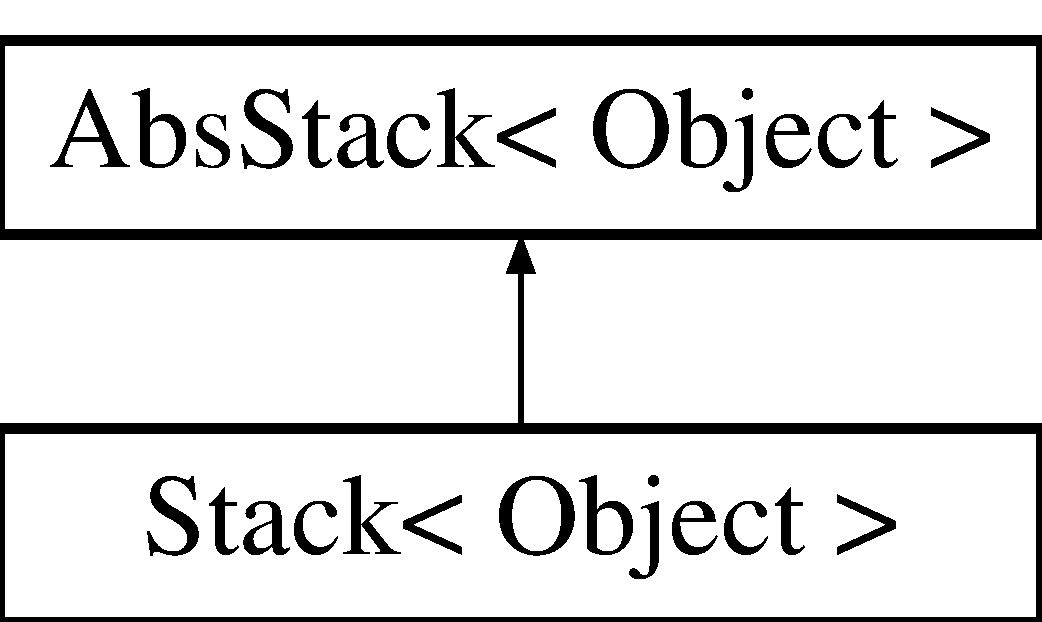
\includegraphics[height=2.000000cm]{classStack}
\end{center}
\end{figure}
\subsection*{Public Member Functions}
\begin{DoxyCompactItemize}
\item 
\hyperlink{classStack_a78a698445d1ac0e1bb2d2678c3e6b4df}{Stack} ()\hypertarget{classStack_a78a698445d1ac0e1bb2d2678c3e6b4df}{}\label{classStack_a78a698445d1ac0e1bb2d2678c3e6b4df}

\begin{DoxyCompactList}\small\item\em Constructor that initializes all attributes. \end{DoxyCompactList}\item 
\hyperlink{classStack_a853c2cc752287e206ea4d759f7baa211}{$\sim$\+Stack} ()\hypertarget{classStack_a853c2cc752287e206ea4d759f7baa211}{}\label{classStack_a853c2cc752287e206ea4d759f7baa211}

\begin{DoxyCompactList}\small\item\em Destructor. \end{DoxyCompactList}\item 
void \hyperlink{classStack_a7a7712fc7e216d9a5ebdff5e2eb82e64}{push} (const Object \&x)\hypertarget{classStack_a7a7712fc7e216d9a5ebdff5e2eb82e64}{}\label{classStack_a7a7712fc7e216d9a5ebdff5e2eb82e64}

\begin{DoxyCompactList}\small\item\em Insert element. \end{DoxyCompactList}\item 
const Object \& \hyperlink{classStack_a3057daa6cff18f7335afe5a1e3f3fd04}{pop} ()
\begin{DoxyCompactList}\small\item\em Remove element. \end{DoxyCompactList}\item 
const Object \& \hyperlink{classStack_a22b3d15b5604db3175589ade35f9a9c9}{top} () const 
\begin{DoxyCompactList}\small\item\em Takes the element at the top. \end{DoxyCompactList}\item 
bool \hyperlink{classStack_ae11870056b681ec3362faca36d6910ec}{empty} () const 
\begin{DoxyCompactList}\small\item\em Tells if the stack is empty. \end{DoxyCompactList}\item 
void \hyperlink{classStack_ac209ae083b7050deb2139f412f9b3861}{clear} ()\hypertarget{classStack_ac209ae083b7050deb2139f412f9b3861}{}\label{classStack_ac209ae083b7050deb2139f412f9b3861}

\begin{DoxyCompactList}\small\item\em Clear stack. \end{DoxyCompactList}\end{DoxyCompactItemize}
\subsection*{Private Member Functions}
\begin{DoxyCompactItemize}
\item 
void \hyperlink{classStack_aa0b9a1c9447e1abaa6e53c84b6a9aaa8}{double\+Data} ()
\end{DoxyCompactItemize}
\subsection*{Private Attributes}
\begin{DoxyCompactItemize}
\item 
int \hyperlink{classStack_aa665dd77e374b82bb86e1fce27308439}{capacity}
\item 
int \hyperlink{classStack_a474893fc0e2f8f87ccd70c09d022439c}{top\+Index}
\item 
Object $\ast$ \hyperlink{classStack_a3d78e7aef171483f22406e598892b7a2}{data}
\end{DoxyCompactItemize}
\subsection*{Static Private Attributes}
\begin{DoxyCompactItemize}
\item 
static const int \hyperlink{classStack_ace70f66cadde9cb3a090e6915eb529aa}{D\+E\+F\+\_\+\+C\+A\+P\+A\+C\+I\+TY} = 50
\end{DoxyCompactItemize}


\subsection{Detailed Description}
\subsubsection*{template$<$typename Object$>$\\*
class Stack$<$ Object $>$}

Implementation of a stack. 

Implemented with a simple array, dinamically reallocated when necessary. \begin{DoxyAuthor}{Authors}
Vitor Rodrigues \hyperlink{namespaceGreati}{Greati}, Vinicius Campos Tinoco Ribeiro 
\end{DoxyAuthor}
\begin{DoxyVersion}{Version}
1.\+0 
\end{DoxyVersion}


\subsection{Member Function Documentation}
\index{Stack@{Stack}!double\+Data@{double\+Data}}
\index{double\+Data@{double\+Data}!Stack@{Stack}}
\subsubsection[{double\+Data()}]{\setlength{\rightskip}{0pt plus 5cm}template$<$typename Object $>$ void {\bf Stack}$<$ Object $>$\+::double\+Data (
\begin{DoxyParamCaption}
{}
\end{DoxyParamCaption}
)\hspace{0.3cm}{\ttfamily [private]}}\hypertarget{classStack_aa0b9a1c9447e1abaa6e53c84b6a9aaa8}{}\label{classStack_aa0b9a1c9447e1abaa6e53c84b6a9aaa8}
Doubles the capacity when necessary. \index{Stack@{Stack}!empty@{empty}}
\index{empty@{empty}!Stack@{Stack}}
\subsubsection[{empty() const }]{\setlength{\rightskip}{0pt plus 5cm}template$<$typename Object $>$ bool {\bf Stack}$<$ Object $>$\+::empty (
\begin{DoxyParamCaption}
{}
\end{DoxyParamCaption}
) const\hspace{0.3cm}{\ttfamily [virtual]}}\hypertarget{classStack_ae11870056b681ec3362faca36d6910ec}{}\label{classStack_ae11870056b681ec3362faca36d6910ec}


Tells if the stack is empty. 

\begin{DoxyReturn}{Returns}
true, if it\textquotesingle{}s empty. 
\end{DoxyReturn}


Implements \hyperlink{classAbsStack}{Abs\+Stack$<$ Object $>$}.

\index{Stack@{Stack}!pop@{pop}}
\index{pop@{pop}!Stack@{Stack}}
\subsubsection[{pop()}]{\setlength{\rightskip}{0pt plus 5cm}template$<$typename Object $>$ const Object\& {\bf Stack}$<$ Object $>$\+::pop (
\begin{DoxyParamCaption}
{}
\end{DoxyParamCaption}
)\hspace{0.3cm}{\ttfamily [virtual]}}\hypertarget{classStack_a3057daa6cff18f7335afe5a1e3f3fd04}{}\label{classStack_a3057daa6cff18f7335afe5a1e3f3fd04}


Remove element. 

\begin{DoxyReturn}{Returns}
A reference to the removed data. 
\end{DoxyReturn}


Implements \hyperlink{classAbsStack}{Abs\+Stack$<$ Object $>$}.

\index{Stack@{Stack}!top@{top}}
\index{top@{top}!Stack@{Stack}}
\subsubsection[{top() const }]{\setlength{\rightskip}{0pt plus 5cm}template$<$typename Object $>$ const Object\& {\bf Stack}$<$ Object $>$\+::top (
\begin{DoxyParamCaption}
{}
\end{DoxyParamCaption}
) const\hspace{0.3cm}{\ttfamily [virtual]}}\hypertarget{classStack_a22b3d15b5604db3175589ade35f9a9c9}{}\label{classStack_a22b3d15b5604db3175589ade35f9a9c9}


Takes the element at the top. 

\begin{DoxyReturn}{Returns}
A reference to the element. 
\end{DoxyReturn}


Implements \hyperlink{classAbsStack}{Abs\+Stack$<$ Object $>$}.



\subsection{Member Data Documentation}
\index{Stack@{Stack}!capacity@{capacity}}
\index{capacity@{capacity}!Stack@{Stack}}
\subsubsection[{capacity}]{\setlength{\rightskip}{0pt plus 5cm}template$<$typename Object $>$ int {\bf Stack}$<$ Object $>$\+::capacity\hspace{0.3cm}{\ttfamily [private]}}\hypertarget{classStack_aa665dd77e374b82bb86e1fce27308439}{}\label{classStack_aa665dd77e374b82bb86e1fce27308439}
Size in memory. \index{Stack@{Stack}!data@{data}}
\index{data@{data}!Stack@{Stack}}
\subsubsection[{data}]{\setlength{\rightskip}{0pt plus 5cm}template$<$typename Object $>$ Object$\ast$ {\bf Stack}$<$ Object $>$\+::data\hspace{0.3cm}{\ttfamily [private]}}\hypertarget{classStack_a3d78e7aef171483f22406e598892b7a2}{}\label{classStack_a3d78e7aef171483f22406e598892b7a2}
Pointer to data. \index{Stack@{Stack}!D\+E\+F\+\_\+\+C\+A\+P\+A\+C\+I\+TY@{D\+E\+F\+\_\+\+C\+A\+P\+A\+C\+I\+TY}}
\index{D\+E\+F\+\_\+\+C\+A\+P\+A\+C\+I\+TY@{D\+E\+F\+\_\+\+C\+A\+P\+A\+C\+I\+TY}!Stack@{Stack}}
\subsubsection[{D\+E\+F\+\_\+\+C\+A\+P\+A\+C\+I\+TY}]{\setlength{\rightskip}{0pt plus 5cm}template$<$typename Object $>$ const int {\bf Stack}$<$ Object $>$\+::D\+E\+F\+\_\+\+C\+A\+P\+A\+C\+I\+TY = 50\hspace{0.3cm}{\ttfamily [static]}, {\ttfamily [private]}}\hypertarget{classStack_ace70f66cadde9cb3a090e6915eb529aa}{}\label{classStack_ace70f66cadde9cb3a090e6915eb529aa}
Default capacity. \index{Stack@{Stack}!top\+Index@{top\+Index}}
\index{top\+Index@{top\+Index}!Stack@{Stack}}
\subsubsection[{top\+Index}]{\setlength{\rightskip}{0pt plus 5cm}template$<$typename Object $>$ int {\bf Stack}$<$ Object $>$\+::top\+Index\hspace{0.3cm}{\ttfamily [private]}}\hypertarget{classStack_a474893fc0e2f8f87ccd70c09d022439c}{}\label{classStack_a474893fc0e2f8f87ccd70c09d022439c}
Points to the top of the stack. 

The documentation for this class was generated from the following file\+:\begin{DoxyCompactItemize}
\item 
include/stack.\+h\end{DoxyCompactItemize}

\hypertarget{structBares_1_1Token}{}\section{Bares\+:\+:Token Struct Reference}
\label{structBares_1_1Token}\index{Bares\+::\+Token@{Bares\+::\+Token}}


Struct that represents each element inside an expression. It can be an operand or an operator.  




{\ttfamily \#include $<$bares.\+h$>$}

\subsection*{Public Member Functions}
\begin{DoxyCompactItemize}
\item 
\hyperlink{structBares_1_1Token_afefce0c2a9140f499b2bc91a5b383d0c}{Token} ()\hypertarget{structBares_1_1Token_afefce0c2a9140f499b2bc91a5b383d0c}{}\label{structBares_1_1Token_afefce0c2a9140f499b2bc91a5b383d0c}

\begin{DoxyCompactList}\small\item\em Basic constructor. \end{DoxyCompactList}\item 
\hyperlink{structBares_1_1Token_ab70f4505f1bc9a1fae540b6198e28b23}{Token} (int \+\_\+column, \hyperlink{classBares_a656cd507b0ddaa049dc7e6548459b6d8}{Type\+Symbol} \+\_\+type, string \+\_\+symbol=\char`\"{}\char`\"{})\hypertarget{structBares_1_1Token_ab70f4505f1bc9a1fae540b6198e28b23}{}\label{structBares_1_1Token_ab70f4505f1bc9a1fae540b6198e28b23}

\begin{DoxyCompactList}\small\item\em Constructor that accepts all attributes and initializes them. Makes token creation a lot easier. \end{DoxyCompactList}\end{DoxyCompactItemize}
\subsection*{Public Attributes}
\begin{DoxyCompactItemize}
\item 
int \hyperlink{structBares_1_1Token_af3adba034744030cd8179d3627098b48}{column}
\item 
\hyperlink{classBares_a656cd507b0ddaa049dc7e6548459b6d8}{Type\+Symbol} \hyperlink{structBares_1_1Token_a64dd409f656e8345531df4025986be40}{type}
\item 
string \hyperlink{structBares_1_1Token_a84b0d3edd9f59ac058c494b007770578}{symbol}
\end{DoxyCompactItemize}


\subsection{Detailed Description}
Struct that represents each element inside an expression. It can be an operand or an operator. 

\subsection{Member Data Documentation}
\index{Bares\+::\+Token@{Bares\+::\+Token}!column@{column}}
\index{column@{column}!Bares\+::\+Token@{Bares\+::\+Token}}
\subsubsection[{column}]{\setlength{\rightskip}{0pt plus 5cm}int Bares\+::\+Token\+::column}\hypertarget{structBares_1_1Token_af3adba034744030cd8179d3627098b48}{}\label{structBares_1_1Token_af3adba034744030cd8179d3627098b48}
Where the token starts in the original expression. \index{Bares\+::\+Token@{Bares\+::\+Token}!symbol@{symbol}}
\index{symbol@{symbol}!Bares\+::\+Token@{Bares\+::\+Token}}
\subsubsection[{symbol}]{\setlength{\rightskip}{0pt plus 5cm}string Bares\+::\+Token\+::symbol}\hypertarget{structBares_1_1Token_a84b0d3edd9f59ac058c494b007770578}{}\label{structBares_1_1Token_a84b0d3edd9f59ac058c494b007770578}
\hyperlink{structBares_1_1Token}{Token}\textquotesingle{}s content. \index{Bares\+::\+Token@{Bares\+::\+Token}!type@{type}}
\index{type@{type}!Bares\+::\+Token@{Bares\+::\+Token}}
\subsubsection[{type}]{\setlength{\rightskip}{0pt plus 5cm}{\bf Type\+Symbol} Bares\+::\+Token\+::type}\hypertarget{structBares_1_1Token_a64dd409f656e8345531df4025986be40}{}\label{structBares_1_1Token_a64dd409f656e8345531df4025986be40}
\hyperlink{structBares_1_1Token}{Token}\textquotesingle{}s type. 

The documentation for this struct was generated from the following file\+:\begin{DoxyCompactItemize}
\item 
include/bares.\+h\end{DoxyCompactItemize}

\hypertarget{classGreati_1_1Vector}{}\section{Greati\+:\+:Vector$<$ T $>$ Class Template Reference}
\label{classGreati_1_1Vector}\index{Greati\+::\+Vector$<$ T $>$@{Greati\+::\+Vector$<$ T $>$}}


A simple Array\+List implementation.  




{\ttfamily \#include $<$vector.\+h$>$}

\subsection*{Public Member Functions}
\begin{DoxyCompactItemize}
\item 
\hyperlink{classGreati_1_1Vector_a8d5c6c0fe7c2877cd5e01e45560f08f6}{Vector} (int \+\_\+cap=\hyperlink{classGreati_1_1Vector_a4f65eea1b021f9ed7a2e068e9022de5a}{D\+E\+F\+A\+U\+L\+T\+\_\+\+C\+AP})
\begin{DoxyCompactList}\small\item\em Constructor\+: takes the size. \end{DoxyCompactList}\item 
\hyperlink{classGreati_1_1Vector_a7ebef8d1de97be5220843160142b7932}{$\sim$\+Vector} (void)\hypertarget{classGreati_1_1Vector_a7ebef8d1de97be5220843160142b7932}{}\label{classGreati_1_1Vector_a7ebef8d1de97be5220843160142b7932}

\begin{DoxyCompactList}\small\item\em Destructor method. \end{DoxyCompactList}\item 
int \hyperlink{classGreati_1_1Vector_ad8f0b9700c7bf38f5fcca7455dbab180}{size} (void) const \hypertarget{classGreati_1_1Vector_ad8f0b9700c7bf38f5fcca7455dbab180}{}\label{classGreati_1_1Vector_ad8f0b9700c7bf38f5fcca7455dbab180}

\begin{DoxyCompactList}\small\item\em Returns the logical size of the list. \end{DoxyCompactList}\item 
void \hyperlink{classGreati_1_1Vector_a021abdb4453aedab2728052eb44a7719}{fill} (const T \&)\hypertarget{classGreati_1_1Vector_a021abdb4453aedab2728052eb44a7719}{}\label{classGreati_1_1Vector_a021abdb4453aedab2728052eb44a7719}

\begin{DoxyCompactList}\small\item\em Fill vector with a value. \end{DoxyCompactList}\item 
void \hyperlink{classGreati_1_1Vector_a41054b62c64bc913806dbfe6e48352d9}{push\+\_\+back} (const T \&)\hypertarget{classGreati_1_1Vector_a41054b62c64bc913806dbfe6e48352d9}{}\label{classGreati_1_1Vector_a41054b62c64bc913806dbfe6e48352d9}

\begin{DoxyCompactList}\small\item\em Add an element to the end. \end{DoxyCompactList}\item 
T \& \hyperlink{classGreati_1_1Vector_a11bd28b0b2652cb33831c79d2b41a7d7}{operator\mbox{[}$\,$\mbox{]}} (int)\hypertarget{classGreati_1_1Vector_a11bd28b0b2652cb33831c79d2b41a7d7}{}\label{classGreati_1_1Vector_a11bd28b0b2652cb33831c79d2b41a7d7}

\begin{DoxyCompactList}\small\item\em Assig\+At operador. \end{DoxyCompactList}\item 
const T \hyperlink{classGreati_1_1Vector_a96b366520d54a440d27431ba04237c90}{operator\mbox{[}$\,$\mbox{]}} (int) const \hypertarget{classGreati_1_1Vector_a96b366520d54a440d27431ba04237c90}{}\label{classGreati_1_1Vector_a96b366520d54a440d27431ba04237c90}

\begin{DoxyCompactList}\small\item\em At operator. \end{DoxyCompactList}\item 
bool \hyperlink{classGreati_1_1Vector_ae08123134236bcc17848515805877945}{operator==} (const \hyperlink{classGreati_1_1Vector}{Vector} \&) const \hypertarget{classGreati_1_1Vector_ae08123134236bcc17848515805877945}{}\label{classGreati_1_1Vector_ae08123134236bcc17848515805877945}

\begin{DoxyCompactList}\small\item\em Equals operator. \end{DoxyCompactList}\item 
const \hyperlink{classGreati_1_1Vector}{Vector} \& \hyperlink{classGreati_1_1Vector_a001887dfc2edb5a6ddc10f4a4ae24b2b}{operator=} (const \hyperlink{classGreati_1_1Vector}{Vector} \&)\hypertarget{classGreati_1_1Vector_a001887dfc2edb5a6ddc10f4a4ae24b2b}{}\label{classGreati_1_1Vector_a001887dfc2edb5a6ddc10f4a4ae24b2b}

\begin{DoxyCompactList}\small\item\em Assign operator. \end{DoxyCompactList}\item 
const \hyperlink{classGreati_1_1Vector}{Vector} \& \hyperlink{classGreati_1_1Vector_ac7b27acbe4aaf67b2c8834d97473a292}{operator=} (const initializer\+\_\+list$<$ T $>$ \&)\hypertarget{classGreati_1_1Vector_ac7b27acbe4aaf67b2c8834d97473a292}{}\label{classGreati_1_1Vector_ac7b27acbe4aaf67b2c8834d97473a292}

\begin{DoxyCompactList}\small\item\em Assign list operator. \end{DoxyCompactList}\end{DoxyCompactItemize}
\subsection*{Private Member Functions}
\begin{DoxyCompactItemize}
\item 
void \hyperlink{classGreati_1_1Vector_a0401cfad220c754004bc9e23a6678c1b}{double\+Data} ()\hypertarget{classGreati_1_1Vector_a0401cfad220c754004bc9e23a6678c1b}{}\label{classGreati_1_1Vector_a0401cfad220c754004bc9e23a6678c1b}

\begin{DoxyCompactList}\small\item\em Doubles the capacity and keep the data. \end{DoxyCompactList}\end{DoxyCompactItemize}
\subsection*{Private Attributes}
\begin{DoxyCompactItemize}
\item 
T $\ast$ \hyperlink{classGreati_1_1Vector_a95cfc9dbb67abb214cc2516c39c68d23}{vec\+Data}
\item 
int \hyperlink{classGreati_1_1Vector_a037b83266461e0b25f963422533efdf0}{vec\+Size}
\item 
int \hyperlink{classGreati_1_1Vector_a54359e7c9f68cb4ea6cae8be750b989a}{vec\+Capacity}
\end{DoxyCompactItemize}
\subsection*{Static Private Attributes}
\begin{DoxyCompactItemize}
\item 
static const int \hyperlink{classGreati_1_1Vector_a4f65eea1b021f9ed7a2e068e9022de5a}{D\+E\+F\+A\+U\+L\+T\+\_\+\+C\+AP} = 50
\end{DoxyCompactItemize}


\subsection{Detailed Description}
\subsubsection*{template$<$typename T$>$\\*
class Greati\+::\+Vector$<$ T $>$}

A simple Array\+List implementation. 

Array\+List with a few methods, useful for B\+A\+R\+ES project mainly.

\begin{DoxyAuthor}{Author}
Vitor \hyperlink{namespaceGreati}{Greati} 
\end{DoxyAuthor}
\begin{DoxyVersion}{Version}
1.\+1 
\end{DoxyVersion}


\subsection{Constructor \& Destructor Documentation}
\index{Greati\+::\+Vector@{Greati\+::\+Vector}!Vector@{Vector}}
\index{Vector@{Vector}!Greati\+::\+Vector@{Greati\+::\+Vector}}
\subsubsection[{Vector(int \+\_\+cap=\+D\+E\+F\+A\+U\+L\+T\+\_\+\+C\+A\+P)}]{\setlength{\rightskip}{0pt plus 5cm}template$<$typename T$>$ {\bf Greati\+::\+Vector}$<$ T $>$\+::{\bf Vector} (
\begin{DoxyParamCaption}
\item[{int}]{\+\_\+cap = {\ttfamily {\bf D\+E\+F\+A\+U\+L\+T\+\_\+\+C\+AP}}}
\end{DoxyParamCaption}
)\hspace{0.3cm}{\ttfamily [inline]}}\hypertarget{classGreati_1_1Vector_a8d5c6c0fe7c2877cd5e01e45560f08f6}{}\label{classGreati_1_1Vector_a8d5c6c0fe7c2877cd5e01e45560f08f6}


Constructor\+: takes the size. 

As parameter is optional, it can be considered the default constructor. 

\subsection{Member Data Documentation}
\index{Greati\+::\+Vector@{Greati\+::\+Vector}!D\+E\+F\+A\+U\+L\+T\+\_\+\+C\+AP@{D\+E\+F\+A\+U\+L\+T\+\_\+\+C\+AP}}
\index{D\+E\+F\+A\+U\+L\+T\+\_\+\+C\+AP@{D\+E\+F\+A\+U\+L\+T\+\_\+\+C\+AP}!Greati\+::\+Vector@{Greati\+::\+Vector}}
\subsubsection[{D\+E\+F\+A\+U\+L\+T\+\_\+\+C\+AP}]{\setlength{\rightskip}{0pt plus 5cm}template$<$typename T$>$ const int {\bf Greati\+::\+Vector}$<$ T $>$\+::D\+E\+F\+A\+U\+L\+T\+\_\+\+C\+AP = 50\hspace{0.3cm}{\ttfamily [static]}, {\ttfamily [private]}}\hypertarget{classGreati_1_1Vector_a4f65eea1b021f9ed7a2e068e9022de5a}{}\label{classGreati_1_1Vector_a4f65eea1b021f9ed7a2e068e9022de5a}
The default capacity of the list. \index{Greati\+::\+Vector@{Greati\+::\+Vector}!vec\+Capacity@{vec\+Capacity}}
\index{vec\+Capacity@{vec\+Capacity}!Greati\+::\+Vector@{Greati\+::\+Vector}}
\subsubsection[{vec\+Capacity}]{\setlength{\rightskip}{0pt plus 5cm}template$<$typename T$>$ int {\bf Greati\+::\+Vector}$<$ T $>$\+::vec\+Capacity\hspace{0.3cm}{\ttfamily [private]}}\hypertarget{classGreati_1_1Vector_a54359e7c9f68cb4ea6cae8be750b989a}{}\label{classGreati_1_1Vector_a54359e7c9f68cb4ea6cae8be750b989a}
Size of the list in memory. \index{Greati\+::\+Vector@{Greati\+::\+Vector}!vec\+Data@{vec\+Data}}
\index{vec\+Data@{vec\+Data}!Greati\+::\+Vector@{Greati\+::\+Vector}}
\subsubsection[{vec\+Data}]{\setlength{\rightskip}{0pt plus 5cm}template$<$typename T$>$ T$\ast$ {\bf Greati\+::\+Vector}$<$ T $>$\+::vec\+Data\hspace{0.3cm}{\ttfamily [private]}}\hypertarget{classGreati_1_1Vector_a95cfc9dbb67abb214cc2516c39c68d23}{}\label{classGreati_1_1Vector_a95cfc9dbb67abb214cc2516c39c68d23}
Pointer to the data. \index{Greati\+::\+Vector@{Greati\+::\+Vector}!vec\+Size@{vec\+Size}}
\index{vec\+Size@{vec\+Size}!Greati\+::\+Vector@{Greati\+::\+Vector}}
\subsubsection[{vec\+Size}]{\setlength{\rightskip}{0pt plus 5cm}template$<$typename T$>$ int {\bf Greati\+::\+Vector}$<$ T $>$\+::vec\+Size\hspace{0.3cm}{\ttfamily [private]}}\hypertarget{classGreati_1_1Vector_a037b83266461e0b25f963422533efdf0}{}\label{classGreati_1_1Vector_a037b83266461e0b25f963422533efdf0}
Logical size of the list. 

The documentation for this class was generated from the following files\+:\begin{DoxyCompactItemize}
\item 
include/vector.\+h\item 
src/vector.\+cpp\end{DoxyCompactItemize}

%--- End generated contents ---

% Index
\backmatter
\newpage
\phantomsection
\clearemptydoublepage
\addcontentsline{toc}{chapter}{Index}
\printindex

\end{document}
